
\section{\label{sec:calculusErrorAnalysis}Analisis Galat}

\subsection{Galat pada Rumus Turunan Pertama}

Pada bagian \ref{sec:polynomialLagrange}, kita memperoleh bahwa jika
$f$ memiliki turunan yang cukup, maka selisih antara $f$ dan $P_{n}$,
yaitu polinom interpolasi berderajat paling tinggi $n$, diberikan
oleh persamaan \ref{eq:lagrangeInterpolatingPolynomialError} \vpageref{eq:lagrangeInterpolatingPolynomialError},
yang disalin di sini untuk memudahkan:
\[
f(x)-P_{n}(x)=\frac{f^{(n+1)}(\xi_{x})}{(n+1)!}(x-x_{0})(x-x_{1})\cdots(x-x_{n}).
\]
Kita dapat menggunakan rumus ini untuk menurunkan rumus ringkas bagi
galat dalam menghampiri $f'(x)$ dengan $P_{n}'(x)$.

Seperti yang dilakukan pada bagian \ref{sec:polynomialLagrange},
misalkan $n\geq1$ dan $x_{0},x_{1},\ldots,x_{n}$ berjumlah $n$
ditambah satu dan semuanya merupakan bilangan real yang berbeda. Tetapkan
$w(x)=(x-x_{0})(x-x_{1})\cdots(x-x_{n})$, $a=\min(x_{0},\ldots,x_{n},x)$,
serta $b=\max(x_{0},\ldots,x_{n},x)$. Dari persamaan \ref{eq:lagrangeInterpolatingPolynomialError},
kita mengetahui bahwa, dengan mengasumsikan $f$ memiliki $n+1$ turunan
pada $(a,b)$ dan $f',f'',\ldots,f^{(n)}$ semuanya kontinu pada $[a,b]$,
untuk setiap $x\in[a,b]$, berlaku

\[
f(x)-P_{n}(x)=\frac{f^{(n+1)}(\xi_{x})}{(n+1)!}w(x)
\]
untuk suatu $\xi_{x}\in(a,b)$. Oleh karena itu,
\[
f'(x)-P_{n}'(x)=\frac{d}{dx}\left[\frac{f^{(n+1)}(\xi_{x})}{(n+1)!}\right]w(x)+\frac{f^{(n+1)}(\xi_{x})}{(n+1)!}w'(x).
\]
Karena $w$ bernilai nol di setiap simpul, rumus ini menjadi lebih
sederhana ketika $x$ merupakan simpul. Tanpa mengurangi keumuman,
kita mengevaluasinya pada $x=x_{0}$ dan memperoleh 
\[
f'(x_{0})-P_{n}'(x_{0})=\frac{f^{(n+1)}(\xi_{x_{0}})}{(n+1)!}w'(x_{0}).
\]
Mulai dari sini, rumus galat ini hanya berlaku pada sebuah simpul!
Ungkapan terakhir ini dapat disederhanakan lebih lanjut dengan memperhatikan
bahwa 
\[
w'(x)=\sum_{i=0}^{n}\prod_{\substack{j=0\\
i\neq j
}
}^{n}(x-x_{j})=\sum_{i=0}^{n}p_{i}(x),
\]
dengan $p_{i}$ sebagaimana didefinisikan untuk persamaan \ref{eq:lagrangeInterpolatingPolynomial}
\vpageref{eq:lagrangeInterpolatingPolynomial}. Namun, $p_{i}(x_{0})=0$
untuk semua $i$ kecuali $i=0$, sehingga
\[
w'(x_{0})=p_{0}(x_{0})=(x_{0}-x_{1})(x_{0}-x_{2})\cdots(x_{0}-x_{n}).
\]
Dengan menyubstitusikan ungkapan untuk $w'$ ini, kita memperoleh
rumus galat turunan pertama
\[
f'(x_{0})-P_{n}'(x_{0})=\frac{f^{(n+1)}(\xi_{x_{0}})}{(n+1)!}(x_{0}-x_{1})(x_{0}-x_{2})\cdots(x_{0}-x_{n}).
\]
Lakukan substitusi $x_{0}+\theta_{i}h$ untuk $x_{i}$, $i=1,2,\ldots,n$,
agar diperoleh rumus dalam bentuk $h$ dan $\theta_{i}$:
\[
f'(x_{0})-P_{n}'(x_{0})=\frac{f^{(n+1)}(\xi_{x_{0}})}{(n+1)!}(-\theta_{1}h)(-\theta_{2}h)\cdots(-\theta_{n}h).
\]
Rumus galat ini masih dapat sedikit disederhanakan:
\begin{equation}
f'(x_{0})-P_{n}'(x_{0})=\frac{f^{(n+1)}(\xi)}{(n+1)!}\theta_{1}\theta_{2}\cdots\theta_{n}(-h)^{n}.\label{eq:firstDerivErrorSimplified}
\end{equation}

Untuk stensil

\begin{center}
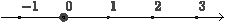
\includegraphics[scale=2]{figures/calculus-errors07},
\par\end{center}

\noindent$n=4$, $\theta_{1}=-1$, $\theta_{2}=1$, $\theta_{3}=2$,
dan $\theta_{4}=3$, sehingga galat dalam menghitung $f'$ pada stensil
ini adalah
\[
\frac{f^{(5)}(\xi)}{120}(-1)(1)(2)(3)(-h)^{4}=-\frac{f^{(5)}(\xi)}{20}h^{4}.
\]
Suku-suku galat untuk turunan pertama pada stensil lain dihitung dengan
cara serupa, asalkan turunannya dievaluasi di sebuah simpul. Tabel
\ref{tab:firstDerivativeFormulas} merangkum beberapa rumus turunan
pertama yang umum, termasuk suku galatnya.

Perhatikan bahwa suku galat memuat $(x_{0}-x_{1})(x_{0}-x_{2})\cdots(x_{0}-x_{n})$
sebagai faktor, yaitu hasil kali semua selisih antara titik evaluasi
dan simpul-simpul lainnya. Jika selisih antara titik evaluasi dan
simpul-simpul lain kecil, hasil kalinya juga kecil. Oleh karena itu,
rumus hampiran turunan pertama umumnya lebih akurat bila titik evaluasi
terletak di tengah di antara simpul-simpul. Dengan demikian, kita
dapat memperkirakan bahwa rumus turunan pertama yang melibatkan simpul
$x_{0}<x_{1}<x_{2}$ akan lebih akurat ketika titik evaluasinya $x_{1}$
daripada ketika titik evaluasinya $x_{0}$ atau $x_{2}$. Hal yang
sama berlaku untuk rumus turunan orde lebih tinggi. Semakin dekat
titik evaluasi ke tengah, semakin akurat hampirannya.

\subsection{Galat pada Rumus Lain\label{subsec:derivativeError}}

Kita mungkin tergoda untuk berpikir bahwa kita cukup mengulangi prosedur
yang digunakan untuk turunan pertama, dengan mengambil turunan kedua
dari $f(x)-P_{n}(x)=\frac{f^{(n+1)}(\xi_{x})}{(n+1)!}w(x)$ untuk
menemukan galat pada taksiran turunan kedua, dan turunan ketiga dari
$f(x)-P_{n}(x)=\frac{f^{(n+1)}(\xi_{x})}{(n+1)!}w(x)$ untuk menemukan
galat pada taksiran turunan ketiga, dan seterusnya. Sayangnya, masalahnya
tidak sesederhana itu. Turunan orde lebih tinggi dari $f(x)-P_{n}(x)=\frac{f^{(n+1)}(\xi_{x})}{(n+1)!}w(x)$
melibatkan turunan dari faktor $\frac{f^{(n+1)}(\xi_{x})}{(n+1)!}$
yang tidak bernilai nol bahkan ketika $x$ merupakan simpul. Karena
$\xi_{x}$ sama sekali tidak diketahui, turunannya pun tidak diketahui
sehingga pendekatan ini tidak dapat digunakan.

Namun, ada metode umum untuk menentukan suku galat yang \textit{cukup
baik} bagi sembarang rumus turunan maupun integral. Setiap evaluasi
$f$ dalam hampiran kita ganti dengan deret Taylor yang dikembangkan
di sekitar $x_{0}$ lalu kita sederhanakan. Ini menghasilkan ungkapan
bagi hampiran dalam bentuk $f(x_{0})$, $f'(x_{0})$, $f''(x_{0})$,
dan seterusnya. Kita membandingkan ungkapan itu dengan representasi
deret Taylor dari besaran yang ditaksir. Selisih keduanya adalah galat.
Ringkasnya, hanya itu. Menyusun argumen yang ketat bagi metode ini
memerlukan kehati-hatian dan layak dibahas melalui sebuah contoh.
Kita memperagakan metode ini untuk hampiran turunan pertama pada stensil

\begin{center}
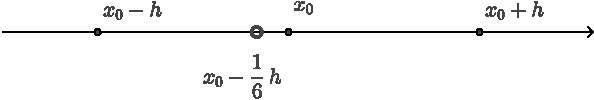
\includegraphics{figures/calculus-rudiments01}.
\par\end{center}

\noindent Sekali lagi, kita memilih stensil ini bukan karena stensil
tersebut berguna secara umum, melainkan untuk menekankan bahwa \textit{metodenya}
berguna secara umum. 

Pada subbagian \ref{subsec:Derivatives} \vpageref{subsec:Derivatives},
kita menurunkan hampiran
\begin{equation}
f'\left(x_{0}-\frac{1}{6}h\right)\approx\frac{-2f(x_{0}-h)+f(x_{0})+f(x_{0}+h)}{3h}.\label{eq:generalApprox}
\end{equation}
Ruas kiri, yaitu besaran yang dihampiri, dalam bentuk deret Taylor
adalah
\[
f'\left(x_{0}-\frac{1}{6}h\right)=f'(x_{0})-\frac{1}{6}hf''(x_{0})+\frac{1}{72}h^{2}f'''(x_{0})-\frac{1}{1296}h^{3}f^{(4)}(x_{0})+\cdots.
\]
Suku-suku pada ruas kanan, yaitu hampirannya, dalam bentuk deret Taylor
adalah
\begin{eqnarray*}
f(x_{0}-h) & = & f(x_{0})-hf'(x_{0})+\frac{1}{2}h^{2}f''(x_{0})-\frac{1}{6}h^{3}f'''(x_{0})+\frac{1}{24}h^{4}f^{(4)}(x_{0})-\cdots\\
f(x_{0}) & = & f(x_{0})\\
f(x_{0}+h) & = & f(x_{0})+hf'(x_{0})+\frac{1}{2}h^{2}f''(x_{0})+\frac{1}{6}h^{3}f'''(x_{0})+\frac{1}{24}h^{4}f^{(4)}(x_{0})+\cdots.
\end{eqnarray*}
Sekarang kita menyubstitusikan deret-deret Taylor ini ke ruas kanan
persamaan \ref{eq:generalApprox} lalu menyederhanakannya. Untuk memudahkan
aljabar, kita mulai dengan menjumlahkan $-2f(x_{0}-h)+f(x_{0})+f(x_{0}+h)$:

\begin{center}
\begin{tabular}{rcl}
$-2f(x_{0}-h)$ & $=$ & $-2f(x_{0})+2hf'(x_{0})-h^{2}f''(x_{0})+\frac{1}{3}h^{3}f'''(x_{0})-\frac{1}{12}h^{4}f^{(4)}(x_{0})-\cdots$\tabularnewline
$f(x_{0})$ & $=$ & $f(x_{0})$\tabularnewline
$f(x_{0}+h)$ & $=$ & $f(x_{0})+hf'(x_{0})+\frac{1}{2}h^{2}f''(x_{0})+\frac{1}{6}h^{3}f'''(x_{0})+\frac{1}{24}h^{4}f^{(4)}(x_{0})+\cdots$\tabularnewline
\hline 
$-2f(x_{0}-h)+f(x_{0})+f(x_{0}+h)$ & $=$ & $3hf'(x_{0})-\frac{1}{2}h^{2}f''(x_{0})+\frac{1}{2}h^{3}f'''(x_{0})-\frac{1}{24}h^{4}f^{(4)}(x_{0})+\cdots$.\tabularnewline
\end{tabular}
\par\end{center}

\noindent Dengan demikian, kita memperoleh 
\begin{eqnarray*}
\frac{-2f(x_{0}-h)+f(x_{0})+f(x_{0}+h)}{3h} & = & \frac{3hf'(x_{0})-\frac{1}{2}h^{2}f''(x_{0})+\frac{1}{2}h^{3}f'''(x_{0})-\frac{1}{24}h^{4}f^{(4)}(x_{0})+\cdots}{3h}\\
 & = & f'(x_{0})-\frac{1}{6}hf''(x_{0})+\frac{1}{6}h^{2}f'''(x_{0})-\frac{1}{72}h^{3}f^{(4)}(x_{0})+\cdots.
\end{eqnarray*}
Untuk galat, $e(h)=f'\left(x_{0}-\frac{1}{6}h\right)-\frac{-2f(x_{0}-h)+f(x_{0})+f(x_{0}+h)}{3h}$,
selanjutnya kita peroleh

\[
\begin{gathered}\left(f'(x_{0})-\frac{1}{6}hf''(x_{0})+\frac{1}{72}h^{2}f'''(x_{0})-\frac{1}{1296}h^{3}f^{(4)}(x_{0})+\cdots\right)\\
\qquad-\left(f'(x_{0})-\frac{1}{6}hf''(x_{0})+\frac{1}{6}h^{2}f'''(x_{0})-\frac{1}{72}h^{3}f^{(4)}(x_{0})+\cdots\right)\\
=-\frac{11}{72}h^{2}f'''(x_{0})+\frac{17}{1296}h^{3}f^{(4)}(x_{0})+\cdots.\qquad\qquad\qquad\qquad\qquad
\end{gathered}
\]
Sebelum melanjutkan, kita perlu membahas notasi O besar\index{O besar}
dalam konteks ini. \index{kekonvergenan!laju} Untuk fungsi $g(h)$
yang memenuhi ${\displaystyle \lim_{h\to0}g(h)=0}$, $p(h)=O(g(h))$
berarti bahwa $|p(h)|\leq M|g(h)|$ untuk suatu konstanta $M$ dan
$h$ yang cukup kecil. Dengan kata lain, besar $p(h)$ dibatasi oleh
besar suatu kelipatan konstan dari $g(h)$. Bandingkan dengan penggunaan
notasi O besar dalam konteks barisan konvergen pada bagian \ref{sec:Speed}. 

Dalam situasi ini, perhitungan kita menunjukkan bahwa galat berbentuk
$O(h^{2}f'''(\xi_{h}))$, yaitu bentuk suku tersisa dengan pangkat
paling rendah. Artinya, $|e(h)|\leq M|h^{2}f'''(\xi_{h})|$ untuk
suatu konstanta $M$ dan $h$ yang cukup kecil, tetapi kita belum
memiliki bukti yang ketat untuk fakta tersebut. Anggaplah apa yang
telah dilakukan sejauh ini sebagai tahap penemuan.

Sekarang kita perlu membuktikan bahwa terdapat $M$ sedemikian rupa
sehingga $|e(h)|\leq M|h^{2}f'''(\xi_{h})|$ berlaku untuk $h$ yang
cukup kecil. Dari perhitungan di atas kita tahu bahwa suku-suku $f'''$
tidak saling meniadakan, jadi kita kembali dan memotong semua deret
Taylor setelah suku $f''$, mengganti turunan berorde lebih tinggi
dengan suku galat, lalu ``mengulang'' aljabarnya. Dengan demikian,
kita mempunyai
\begin{eqnarray*}
f'\left(x_{0}-\frac{1}{6}h\right) & = & f'(x_{0})-\frac{1}{6}hf''(x_{0})+\frac{1}{72}h^{2}f'''(\xi_{1})\\
f(x_{0}-h) & = & f(x_{0})-hf'(x_{0})+\frac{1}{2}h^{2}f''(x_{0})-\frac{1}{6}h^{3}f'''(\xi_{2})\\
f(x_{0}) & = & f(x_{0})\\
f(x_{0}+h) & = & f(x_{0})+hf'(x_{0})+\frac{1}{2}h^{2}f''(x_{0})+\frac{1}{6}h^{3}f'''(\xi_{3})
\end{eqnarray*}
dengan $\xi_{1}\in(x_{0}-\frac{1}{6}h,x_{0})$, $\xi_{2}\in(x_{0}-h,x_{0})$,
serta $\xi_{3}\in(x_{0},x_{0}+h)$. Ketika sekarang kita menghitung
$e(h)=f'\left(x_{0}-\frac{1}{6}h\right)-\frac{-2f(x_{0}-h)+f(x_{0})+f(x_{0}+h)}{3h}$,
kita tahu bahwa semua suku yang melibatkan $f$, $f'$, serta $f''$
saling meniadakan. Hanya suku yang melibatkan $f'''$ yang tersisa:
\begin{eqnarray*}
e(h) & = & \frac{1}{72}h^{2}f'''(\xi_{1})-\frac{-2(-\frac{1}{6}h^{3}f'''(\xi_{2}))+\frac{1}{6}h^{3}f'''(\xi_{3})}{3h}\\
 & = & \frac{1}{72}h^{2}f'''(\xi_{1})-\frac{1}{9}h^{2}f'''(\xi_{2})-\frac{1}{18}h^{2}f'''(\xi_{3})\\
 & = & \frac{h^{2}}{9}\left[\frac{1}{8}f'''(\xi_{1})-f'''(\xi_{2})-\frac{1}{2}f'''(\xi_{3})\right].
\end{eqnarray*}
Langkah formal terakhir adalah mengubah ungkapan ini ke notasi O besar:
\begin{eqnarray*}
|e(h)| & = & \left|\frac{h^{2}}{9}\left[\frac{1}{8}f'''(\xi_{1})-f'''(\xi_{2})-\frac{1}{2}f'''(\xi_{3})\right]\right|\\
 & \leq & \frac{h^{2}}{9}\left[\left|\frac{1}{8}f'''(\xi_{1})\right|+\left|f'''(\xi_{2})\right|+\left|\frac{1}{2}f'''(\xi_{3})\right|\right]\\
 & \leq & \frac{h^{2}}{9}\cdot\frac{13}{8}\max\left\{ \left|f'''(\xi_{1})\right|,\left|f'''(\xi_{2})\right|,\left|f'''(\xi_{3})\right|\right\} \\
 & = & h^{2}\cdot M\left|f'''(\xi_{h})\right|
\end{eqnarray*}
 untuk suatu $\xi_{h}\in(x_{0}-h,x_{0}+h)$ dan $M=\frac{13}{72}$.
Nilai $\xi_{h}$ adalah $\xi_{1}$, $\xi_{2}$, atau $\xi_{3}$. Kita
menyimpulkan
\[
e(h)=O(h^{2}f'''(\xi_{h})).
\]
Secara umum, $\xi_{h}$ dijamin berada di antara simpul terkecil
dan simpul terbesar. Dalam kasus hampiran integral, titik-titik ujung
integrasi diperlakukan sebagai simpul untuk menentukan letak $\xi_{h}$.
Perhatikan bahwa seluruh perhitungan ini bergantung pada kekontinuan
$f'''(x)$ pada interval antara simpul terkecil dan simpul terbesar.
Tanpa kekontinuan tersebut, teorema Taylor tidak berlaku dan semua
perhitungan setelah ekspansi tidak bermakna.

\subsection{Kuadratur Gauss\index{kuadratur!Gauss}}

Pada akhirnya, keakuratan suatu rumus kalkulus numerik diukur melalui
suku galatnya, suatu besaran berbentuk $O(h^{n}f^{(k)}(\xi_{h}))$.
Jika yang kita perhatikan adalah laju kekonvergenan, kita meninjau
$n$, yaitu pangkat $h$ yang muncul dalam suku galat. Semakin besar
pangkat tersebut, semakin cepat kekonvergenannya. Namun, jika yang
kita perhatikan adalah kelas polinom terbesar yang membuat rumus itu
eksak, kita perlu meninjau nilai $k$, yaitu orde turunan yang muncul
dalam suku galat. Semakin besar $k$, semakin besar pula kelas polinom
yang membuat rumus tersebut eksak. Bahkan, jika suku galat memuat
faktor $f^{(k)}(\xi_{h})$, maka rumus tersebut eksak untuk semua
polinom hingga dan termasuk derajat $k-1$. Implikasi lanjutannya
adalah terdapat polinom berderajat $k$ yang untuknya rumus tersebut
tidak eksak, sebab jika tidak demikian, suku galat akan melibatkan
turunan berorde lebih tinggi. Nilai $k-1$ ini kita sebut derajat
ketelitian. Secara formal, derajat ketelitian\index{derajat ketelitian|see\{ketelitian ! derajat\}}\index{ketelitian!derajat}
suatu rumus kalkulus numerik adalah bilangan bulat $m$ sedemikian
rupa sehingga rumus tersebut eksak untuk semua polinom hingga dan
termasuk derajat $m$ tetapi tidak eksak untuk semua polinom berderajat
$m+1$. Rumus kuadratur Gauss bertujuan memaksimalkan derajat ketelitian
rumus integral. 

Turunan dan integral numerik pada stensil dengan $n+1$ titik yang
telah kita turunkan sejauh ini eksak untuk semua polinom hingga derajat
$n$, sebagaimana mestinya. Derajat ketelitiannya sekurang-kurangnya
$n$. Ternyata, beberapa di antaranya memiliki derajat ketelitian
lebih besar daripada $n$. Pertimbangkan hampiran turunan kedua pada
stensil

\begin{center}
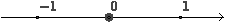
\includegraphics[scale=1.5]{figures/calculus-errors01}.
\par\end{center}

\noindent Stensil ini memiliki tiga titik, jadi kita mengharapkannya
eksak untuk semua polinom hingga derajat 2 (dan memang demikian).
Namun, suku galatnya adalah $O(h^{2}f^{(4)}(\xi_{h}))$, yang menunjukkan
bahwa rumus tersebut eksak untuk semua polinom hingga derajat 3. Jadi,
derajat ketelitiannya sebenarnya 3, bukan 2. Rumus turunan pertama
pada stensil yang sama juga serupa. Walaupun suku galatnya adalah
$\frac{h^{2}}{6}f'''(\xi_{h})$, yang menunjukkan bahwa rumus tersebut
memiliki derajat ketelitian 2 sesuai harapan, rumus itu sendiri hanya
melibatkan dua dari tiga titik yang tersedia! Koefisien $f(x_{0})$
ternyata nol. Dengan demikian, rumus yang sama dapat kita turunkan
dengan menggunakan stensil

\begin{center}
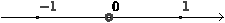
\includegraphics[scale=1.5]{figures/calculus-errors26},
\par\end{center}

\noindent yang hanya memiliki dua titik, tetapi berderajat ketelitian
2. Beberapa beda terpusat lainnya memiliki sifat ini. Rumus Newton-Cotes
dengan jumlah simpul ganjil juga memiliki sifat ini. Derajat ketelitiannya
melampaui perkiraan sebesar satu derajat. Sebelumnya kita mencatat
bahwa titik evaluasi yang terletak di tengah cenderung meningkatkan
keakuratan, dan sekarang kita melihat bahwa peningkatan itu dapat
sangat besar.

Dari pengamatan ini dapat kita simpulkan bahwa bukan hanya jumlah
simpul yang menentukan suku galat suatu rumus kalkulus numerik. Letak
simpul juga penting. Sampai saat ini, kita baru melihat bagaimana
letak simpul memengaruhi hampiran turunan. Kita tahu bahwa menempatkan
titik evaluasi di tengah pada umumnya meningkatkan keakuratan. Sekarang
kita membahas cara menempatkan simpul untuk meningkatkan keakuratan
rumus integral. Namun, gagasan titik evaluasi yang berada di tengah
tidak bermakna dalam konteks ini. Integral tidak memiliki satu titik
evaluasi; integral dihitung pada suatu interval. Yang penting adalah
letak simpul relatif terhadap titik-titik ujung integrasi. Sekarang
kita akan menentukan letak simpul agar derajat ketelitian terbesar
tercapai untuk setiap jumlah simpul tertentu.

Misalkan $G_{n}$ adalah polinom Legendre ke-$n$, yang didefinisikan
secara rekursif oleh 
\begin{eqnarray*}
G_{n+1}(x) & = & \frac{(2n+1)xG_{n}(x)-nG_{n-1}(x)}{n+1}\\
G_{0}(x) & = & 1\\
G_{1}(x) & = & x.
\end{eqnarray*}
Kita menetapkan $\theta_{i}$ sama dengan akar-akar $G_{n}$ untuk
menurunkan rumus kuadratur $n$-titik pada interval $[x_{0}-h,x_{0}+h]$
dengan derajat ketelitian terbesar yang mungkin. Setelah penempatan
simpul dipilih, kita memaksa rumus tersebut eksak bagi polinom hingga
derajat $n-1$, seperti yang kita lakukan sebelumnya. Perbedaannya
kali ini adalah bahwa karena nilai khusus $\theta_{i}$, rumus yang
dihasilkan akan eksak untuk semua polinom hingga derajat $2n-1$.
Ketika simpul ditempatkan pada akar-akar polinom Legendre ke-$n$,
kita memperoleh rumus kuadratur untuk $\int_{x_{0}-h}^{x_{0}+h}f(x)dx$
yang melampaui derajat ketelitian yang diharapkan sebesar $n$, yaitu
jumlah simpul!

Kita memperagakannya untuk $n=1$ dan $n=3$.

\[
G_{1}(x)=x
\]
memiliki satu-satunya akar, $0$. Oleh karena itu, kita mencari rumus
berbentuk 
\[
\int_{x_{0}-h}^{x_{0}+h}f(x)dx\approx a_{0}f(x_{0})
\]
yang eksak untuk polinom hingga derajat $0$. Persamaan tunggal untuk
satu peubah tak diketahui, $a_{0}$, adalah
\[
\int_{x_{0}-h}^{x_{0}+h}(1)dx=a_{0}(1)
\]
atau $2h=a_{0}$. Oleh karena itu, kita memperoleh
\[
\int_{x_{0}-h}^{x_{0}+h}f(x)dx\approx2hf(x_{0}),
\]
yang kita klaim berderajat ketelitian 1, bukan 0. Memang, untuk $f(x)=x-x_{0}$,
\[
\int_{x_{0}-h}^{x_{0}+h}f(x)dx=\left.\frac{1}{2}(x-x_{0})^{2}\right|_{x_{0}-h}^{x_{0}+h}=0
\]
 dan
\[
2hf(x_{0})=2h(x_{0}-x_{0})=0,
\]
sehingga rumus tersebut eksak untuk polinom berderajat satu. Namun,
untuk $f(x)=(x-x_{0})^{2}$,
\[
\int_{x_{0}-h}^{x_{0}+h}f(x)dx=\left.\frac{1}{3}(x-x_{0})^{3}\right|_{x_{0}-h}^{x_{0}+h}=\frac{2}{3}h^{3}
\]
tetapi
\[
2hf(x_{0})=2h(x_{0}-x_{0})^{2}=0,
\]
sehingga rumus tersebut tidak eksak untuk semua polinom berderajat
dua. Jadi, derajat ketelitiannya adalah 1. Perhatikan bahwa rumus
${\displaystyle \int_{x_{0}-h}^{x_{0}+h}f(x)dx\approx2hf(x_{0})}$
setara dengan Aturan Titik Tengah seperti yang tercantum pada Tabel
\ref{tab:integrationFormulas}.

Sekarang
\begin{eqnarray*}
G_{2}(x) & = & \frac{3xG_{1}(x)-G_{0}(x)}{2}\\
 & = & \frac{1}{2}(3x^{2}-1)
\end{eqnarray*}
 sehingga
\begin{eqnarray*}
G_{3}(x) & = & \frac{5xG_{2}(x)-2G_{1}(x)}{3}\\
 & = & \frac{\frac{5}{2}(3x^{3}-x)-2x}{3}\\
 & = & \frac{5(3x^{3}-x)-4x}{6}\\
 & = & \frac{15x^{3}-9x}{6}\\
 & = & \frac{1}{2}(5x^{3}-3x),
\end{eqnarray*}
yang memiliki akar-akar $-\sqrt{\frac{3}{5}},0,\sqrt{\frac{3}{5}}$.
Oleh karena itu, kita mencari rumus berbentuk 
\[
\int_{x_{0}-h}^{x_{0}+h}f(x)dx\approx a_{0}f\left(x_{0}-\sqrt{\frac{3}{5}}h\right)+a_{1}f(x_{0})+a_{2}f\left(x_{0}+\sqrt{\frac{3}{5}}h\right)
\]
yang eksak untuk polinom hingga derajat $2$. Tiga persamaan untuk
tiga peubah tak diketahui tersebut adalah
\begin{eqnarray*}
\int_{x_{0}-h}^{x_{0}+h}(1)dx=2h & = & a_{0}+a_{1}+a_{2}\\
\int_{x_{0}-h}^{x_{0}+h}(x-x_{0})dx=0 & = & -\sqrt{\frac{3}{5}}ha_{0}+\sqrt{\frac{3}{5}}ha_{2}\\
\int_{x_{0}-h}^{x_{0}+h}(x-x_{0})^{2}dx=\frac{2}{3}h^{3} & = & \frac{3}{5}h^{2}a_{0}+\frac{3}{5}h^{2}a_{2}.
\end{eqnarray*}
Solusinya adalah 
\[
a_{0}=a_{2}=\frac{5}{9}h\quad\mbox{dan}\quad a_{1}=\frac{8}{9}h,
\]
sehingga rumus kuadraturnya adalah
\[
\int_{x_{0}-h}^{x_{0}+h}f(x)dx\approx\frac{h}{9}\left[5f\left(x_{0}-\sqrt{\frac{3}{5}}h\right)+8f(x_{0})+5f\left(x_{0}+\sqrt{\frac{3}{5}}h\right)\right].
\]
Rumus ini diturunkan agar eksak untuk polinom hingga derajat 2, sehingga
derajat ketelitiannya sekurang-kurangnya 2. Kita mengklaim bahwa derajat
ketelitiannya sebenarnya 5. Untuk $f(x)=(x-x_{0})^{3}$, 
\[
\int_{x_{0}-h}^{x_{0}+h}f(x)dx=\left.\frac{1}{4}(x-x_{0})^{4}\right|_{x_{0}-h}^{x_{0}+h}=0
\]
 dan
\[
\frac{h}{9}\left[5f\left(x_{0}-\sqrt{\frac{3}{5}}h\right)+8f(x_{0})+5f\left(x_{0}+\sqrt{\frac{3}{5}}h\right)\right]=\frac{h}{9}\left[5\left(-\sqrt{\frac{3}{5}}h\right)^{3}+0+5\left(\sqrt{\frac{3}{5}}h\right)^{3}\right]=0,
\]
sehingga rumus tersebut eksak untuk polinom berderajat tiga. Untuk
$f(x)=(x-x_{0})^{4}$, 
\[
\int_{x_{0}-h}^{x_{0}+h}f(x)dx=\left.\frac{1}{5}(x-x_{0})^{5}\right|_{x_{0}-h}^{x_{0}+h}=\frac{2}{5}h^{5}
\]
 dan
\begin{eqnarray*}
\frac{h}{9}\left[5f\left(x_{0}-\sqrt{\frac{3}{5}}h\right)+8f(x_{0})+5f\left(x_{0}+\sqrt{\frac{3}{5}}h\right)\right] & = & \frac{h}{9}\left[5\left(-\sqrt{\frac{3}{5}}h\right)^{4}+0+5\left(\sqrt{\frac{3}{5}}h\right)^{4}\right]\\
 & = & \frac{5}{9}h\left[\frac{9}{25}h^{4}+\frac{9}{25}h^{4}\right]\\
 & = & \frac{2}{5}h^{5},
\end{eqnarray*}
sehingga rumus tersebut eksak untuk polinom berderajat empat. Untuk
$f(x)=(x-x_{0})^{5}$, 
\[
\int_{x_{0}-h}^{x_{0}+h}f(x)dx=\left.\frac{1}{6}(x-x_{0})^{6}\right|_{x_{0}-h}^{x_{0}+h}=0
\]
 dan
\[
\frac{h}{9}\left[5f\left(x_{0}-\sqrt{\frac{3}{5}}h\right)+8f(x_{0})+5f\left(x_{0}+\sqrt{\frac{3}{5}}h\right)\right]=\frac{h}{9}\left[5\left(-\sqrt{\frac{3}{5}}h\right)^{5}+0+5\left(\sqrt{\frac{3}{5}}h\right)^{5}\right]=0,
\]
sehingga rumus tersebut eksak untuk polinom berderajat lima. Namun,
untuk $f(x)=(x-x_{0})^{6}$, 
\[
\int_{x_{0}-h}^{x_{0}+h}f(x)dx=\left.\frac{1}{7}(x-x_{0})^{7}\right|_{x_{0}-h}^{x_{0}+h}=\frac{2}{7}h^{7}
\]
 dan
\begin{eqnarray*}
\frac{h}{9}\left[5f\left(x_{0}-\sqrt{\frac{3}{5}}h\right)+8f(x_{0})+5f\left(x_{0}+\sqrt{\frac{3}{5}}h\right)\right] & = & \frac{h}{9}\left[5\left(-\sqrt{\frac{3}{5}}h\right)^{6}+0+5\left(\sqrt{\frac{3}{5}}h\right)^{6}\right]\\
 & = & \frac{5}{9}h\left[\frac{27}{125}h^{6}+\frac{27}{125}h^{6}\right]\\
 & = & \frac{3}{25}h^{7},
\end{eqnarray*}
sehingga rumus tersebut tidak eksak untuk semua polinom berderajat
enam. Derajat ketelitiannya adalah 5. Rumus ini tercantum sebagai
rumus kuadratur Gauss kedua pada Tabel \ref{tab:integrationFormulas}. 

Derajat ketelitian setiap rumus kalkulus numerik juga dapat kita tentukan
dengan mengamati bentuk suku galatnya. Jika suku galat berbentuk $O(h^{n}f^{(k)}(\xi_{h}))$,
maka derajat ketelitiannya adalah $k-1$. 

\subsection{Beberapa Rumus Standar}

Tabel \ref{tab:firstDerivativeFormulas}
\begin{table}
\caption{\label{tab:firstDerivativeFormulas}Beberapa rumus turunan pertama
standar.}

\renewcommand{\arraystretch}{2.5}\bigskip 
\centering{}%
\begin{turn}{90}
\begin{tabular}{|c|c|c|}
\multicolumn{1}{c}{Stensil} & \multicolumn{1}{c}{Rumus} & \multicolumn{1}{c}{Nama}\tabularnewline
\hline 
\multicolumn{3}{|c|}{Rumus 2 titik}\tabularnewline
\hline 
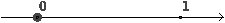
\includegraphics{figures/calculus-errors02} & ${\displaystyle f'(x_{0})=\frac{-f(x_{0})+f(x_{0}+h)}{h}-\frac{h}{2}f''(\xi_{h})}$ & Beda Maju\tabularnewline
\hline 
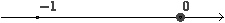
\includegraphics{figures/calculus-errors03} & ${\displaystyle f'(x_{0})=\frac{-f(x_{0}-h)+f(x_{0})}{h}+\frac{h}{2}f''(\xi_{h})}$ & Beda Mundur\tabularnewline
\hline 
\multicolumn{3}{|c|}{Rumus 3 titik}\tabularnewline
\hline 
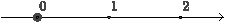
\includegraphics{figures/calculus-errors05} & ${\displaystyle f'(x_{0})=\frac{-3f(x_{0})+4f(x_{0}+h)-f(x_{0}+2h)}{2h}+\frac{h^{2}}{3}f'''(\xi_{h})}$ & Beda Maju\tabularnewline
\hline 
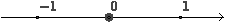
\includegraphics{figures/calculus-errors01} & ${\displaystyle f'(x_{0})=\frac{-f(x_{0}-h)+f(x_{0}+h)}{2h}+\frac{h^{2}}{6}f'''(\xi_{h})}$ & Beda Terpusat\tabularnewline
\hline 
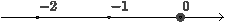
\includegraphics{figures/calculus-errors04} & ${\displaystyle f'(x_{0})=\frac{f(x_{0}-2h)-4f(x_{0}-h)+3f(x_{0})}{2h}+\frac{h^{2}}{3}f'''(\xi_{h})}$ & Beda Mundur\tabularnewline
\hline 
\multicolumn{3}{|c}{Rumus 5 titik}\tabularnewline
\hline 

\includegraphics{figures/calculus-errors08} & ${\displaystyle f'(x_{0})=\frac{-25f(x_{0})+48f(x_{0}+h)-36f(x_{0}+2h)+16f(x_{0}+3h)-3f(x_{0}+4h)}{12h}+\frac{h^{4}}{5}f^{(5)}(\xi_{h})}$ & Beda Maju\tabularnewline
\hline 
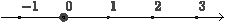
\includegraphics{figures/calculus-errors07} & ${\displaystyle f'(x_{0})=\frac{-3f(x_{0}-h)-10f(x_{0})+18f(x_{0}+h)-6f(x_{0}+2h)+f(x_{0}+3h)}{12h}+\frac{h^{4}}{20}f^{(5)}(\xi_{h})}$ & \tabularnewline
\hline 
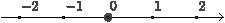
\includegraphics{figures/calculus-errors06} & ${\displaystyle f'(x_{0})=\frac{f(x_{0}-2h)-8f(x_{0}-h)+8f(x_{0}+h)-f(x_{0}+2h)}{12h}+\frac{h^{4}}{30}f^{(5)}(\xi_{h})}$ & Beda Terpusat\tabularnewline
\hline 
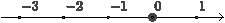
\includegraphics{figures/calculus-errors09} & ${\displaystyle f'(x_{0})=\frac{-f(x_{0}-3h)+6f(x_{0}-2h)-18f(x_{0}-h)+10f(x_{0})+3f(x_{0}+h)}{12h}+\frac{h^{4}}{20}f^{(5)}(\xi_{h})}$ & \tabularnewline
\hline 
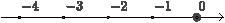
\includegraphics{figures/calculus-errors10} & ${\displaystyle f'(x_{0})=\frac{3f(x_{0}-4h)-16f(x_{0}-3h)+36f(x_{0}-2h)-48f(x_{0}-h)+25f(x_{0})}{12h}+\frac{h^{4}}{5}f^{(5)}(\xi_{h})}$ & Beda Mundur\tabularnewline
\hline 
\end{tabular}
\end{turn}
\end{table}
, \ref{tab:secondDerivativeFormulas}
\begin{table}
\caption{\label{tab:secondDerivativeFormulas}Beberapa rumus turunan kedua.}

\renewcommand{\arraystretch}{2.5}\bigskip 
\centering{}%
\begin{turn}{90}
\begin{tabular}{|c|c|c|}
\multicolumn{1}{c}{Stensil} & \multicolumn{1}{c}{Rumus} & \multicolumn{1}{c}{Nama}\tabularnewline
\hline 
\multicolumn{3}{|c|}{Rumus 3 titik}\tabularnewline
\hline 
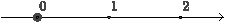
\includegraphics{figures/calculus-errors05} & ${\displaystyle f''(x_{0})=\frac{f(x_{0})-2f(x_{0}+h)+f(x_{0}+2h)}{h^{2}}+O(hf^{(3)}(\xi_{h}))}$ & Beda Maju\tabularnewline
\hline 
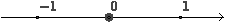
\includegraphics{figures/calculus-errors01} & ${\displaystyle f''(x_{0})=\frac{f(x_{0}-h)-2f(x_{0})+f(x_{0}+h)}{h^{2}}+O(h^{2}f^{(4)}(\xi_{h}))}$ & Beda Terpusat\tabularnewline
\hline 
\multicolumn{3}{|c|}{Rumus 4 titik}\tabularnewline
\hline 
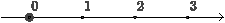
\includegraphics{figures/calculus-errors14} & ${\displaystyle f''(x_{0})=\frac{2f(x_{0})-5f(x_{0}+h)+4f(x_{0}+2h)-f(x_{0}+3h)}{h^{2}}+O(h^{2}f^{(4)}(\xi_{h}))}$ & Beda Maju\tabularnewline
\hline 
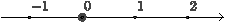
\includegraphics{figures/calculus-errors13} & ${\displaystyle f''(x_{0})=\frac{f(x_{0}-h)-2f(x_{0})+f(x_{0}+h)}{h^{2}}+O(h^{2}f^{(4)}(\xi_{h}))}$ & \tabularnewline
\hline 
\multicolumn{3}{|c}{Rumus 5 titik}\tabularnewline
\hline 

\includegraphics{figures/calculus-errors08} & ${\displaystyle f''(x_{0})=\frac{35f(x_{0})-104f(x_{0}+h)+114f(x_{0}+2h)-56f(x_{0}+3h)+11f(x_{0}+4h)}{12h^{2}}+O(h^{3}f^{(5)}(\xi_{h}))}$ & Beda Maju\tabularnewline
\hline 
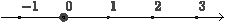
\includegraphics{figures/calculus-errors07} & ${\displaystyle f''(x_{0})=\frac{11f(x_{0}-h)-20f(x_{0})+6f(x_{0}+h)+4f(x_{0}+2h)-f(x_{0}+3h)}{12h^{2}}+O(h^{3}f^{(5)}(\xi_{h}))}$ & \tabularnewline
\hline 
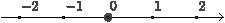
\includegraphics{figures/calculus-errors06} & ${\displaystyle f''(x_{0})=\frac{-f(x_{0}-2h)+16f(x_{0}-h)-30f(x_{0})+16f(x_{0}+h)-f(x_{0}+2h)}{12h^{2}}+O(h^{4}f^{(6)}(\xi_{h}))}$ & Beda Terpusat\tabularnewline
\hline 
\end{tabular}
\end{turn}
\end{table}
, \ref{tab:thirdDerivativeFormulas}
\begin{table}
\caption{\label{tab:thirdDerivativeFormulas}Beberapa rumus turunan ketiga.}

\renewcommand{\arraystretch}{2.5}\bigskip 
\centering{}%
\begin{turn}{90}
\begin{tabular}{|c|c|c|}
\multicolumn{1}{c}{Stensil} & \multicolumn{1}{c}{Rumus} & \multicolumn{1}{c}{Nama}\tabularnewline
\hline 
\multicolumn{3}{|c|}{Rumus 4 titik}\tabularnewline
\hline 
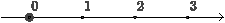
\includegraphics{figures/calculus-errors14} & ${\displaystyle f'''(x_{0})=\frac{-f(x_{0})+3f(x_{0}+h)-3f(x_{0}+2h)+f(x_{0}+3h)}{h^{3}}+O(h)f^{(4)}(\xi_{h})}$ & Beda Maju\tabularnewline
\hline 
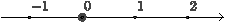
\includegraphics{figures/calculus-errors13} & ${\displaystyle f'''(x_{0})=\frac{-f(x_{0}-h)+3f(x_{0})-3f(x_{0}+h)+f(x_{0}+2h)}{h^{3}}+O(hf^{(4)}(\xi_{h}))}$ & \tabularnewline
\hline 
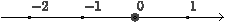
\includegraphics{figures/calculus-errors12} & ${\displaystyle f'''(x_{0})=\frac{-f(x_{0}-2h)+3f(x_{0}-h)-3f(x_{0})+f(x_{0}+h)}{h^{3}}+O(hf^{(4)}(\xi_{h}))}$ & \tabularnewline
\hline 
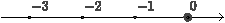
\includegraphics{figures/calculus-errors11} & ${\displaystyle f'''(x_{0})=\frac{-f(x_{0})+3f(x_{0}+h)-3f(x_{0}+2h)+f(x_{0}+3h)}{h^{3}}+O(hf^{(4)}(\xi_{h}))}$ & Beda Mundur\tabularnewline
\hline 
\multicolumn{3}{|c}{Rumus 5 titik}\tabularnewline
\hline 

\includegraphics{figures/calculus-errors08} & ${\displaystyle f'''(x_{0})=\frac{-5f(x_{0})+18f(x_{0}+h)-24f(x_{0}+2h)+14f(x_{0}+3h)-3f(x_{0}+4h)}{2h^{3}}+O(h^{2}f^{(5)}(\xi_{h}))}$ & Beda Maju\tabularnewline
\hline 
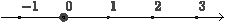
\includegraphics{figures/calculus-errors07} & ${\displaystyle f'''(x_{0})=\frac{-3f(x_{0}-h)+10f(x_{0})-12f(x_{0}+h)+6f(x_{0}+2h)-f(x_{0}+3h)}{2h^{3}}+O(h^{2}f^{(5)}(\xi_{h}))}$ & \tabularnewline
\hline 
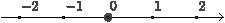
\includegraphics{figures/calculus-errors06} & ${\displaystyle f'''(x_{0})=\frac{-f(x_{0}-2h)+2f(x_{0}-h)-2f(x_{0}+h)+f(x_{0}+2h)}{2h^{3}}+O(h^{2}f^{(5)}(\xi_{h}))}$ & Beda Terpusat\tabularnewline
\hline 
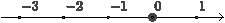
\includegraphics{figures/calculus-errors09} & ${\displaystyle f'''(x_{0})=\frac{f(x_{0}-3h)-6f(x_{0}-2h)+12f(x_{0}-h)-10f(x_{0})+3f(x_{0}+h)}{2h^{3}}+O(h^{2}f^{(5)}(\xi_{h}))}$ & \tabularnewline
\hline 
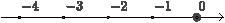
\includegraphics{figures/calculus-errors10} & ${\displaystyle f'''(x_{0})=\frac{3f(x_{0}-4h)-14f(x_{0}-3h)+24f(x_{0}-2h)-18f(x_{0}-h)+5f(x_{0})}{2h^{3}}+O(h^{2}f^{(5)}(\xi_{h}))}$ & Beda Mundur\tabularnewline
\hline 
\end{tabular}
\end{turn}
\end{table}
, dan \ref{tab:integrationFormulas}
\begin{table}
\caption{\label{tab:integrationFormulas}Beberapa rumus integrasi.}

\renewcommand{\arraystretch}{2.5}\bigskip 
\centering{}%
\begin{turn}{90}
\begin{tabular}{|c|c|c|}
\multicolumn{1}{c}{Stensil} & \multicolumn{1}{c}{Rumus} & \multicolumn{1}{c}{Nama}\tabularnewline
\hline 
\multicolumn{3}{|c|}{rumus Newton-Cotes terbuka}\tabularnewline
\hline 
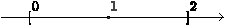
\includegraphics{figures/calculus-errors19} & ${\displaystyle \int_{x_{0}}^{x_{0}+2h}f(x)dx=2hf(x_{0}+h)+O(h^{3}f''(\xi_{h}))}$ & Aturan Titik Tengah\index{aturan titik tengah}\tabularnewline
\hline 
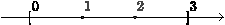
\includegraphics{figures/calculus-errors20} & ${\displaystyle \int_{x_{0}}^{x_{0}+3h}f(x)dx=\frac{3h}{2}\left[f(x_{0}+h)+f(x_{0}+2h)\right]+O(h^{3}f''(\xi_{h}))}$ & \tabularnewline
\hline 
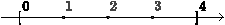
\includegraphics{figures/calculus-errors21} & ${\displaystyle \int_{x_{0}}^{x_{0}+4h}f(x)dx=\frac{4h}{3}\left[2f(x_{0}+h)-f(x_{0}+2h)+2f(x_{0}+3h)\right]+O(h^{5}f^{(4)}(\xi_{h}))}$ & \tabularnewline
\hline 
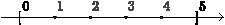
\includegraphics{figures/calculus-errors22} & ${\displaystyle \int_{x_{0}}^{x_{0}+5h}f(x)dx=\frac{5h}{24}\left[11f(x_{0}+h)+f(x_{0}+2h)+f(x_{0}+3h)+11f(x_{0}+4h)\right]+O(h^{5}f^{(4)}(\xi_{h}))}$ & \tabularnewline
\hline 
\multicolumn{3}{|c}{rumus Newton-Cotes tertutup}\tabularnewline
\hline 
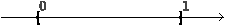
\includegraphics{figures/calculus-errors15} & ${\displaystyle \int_{x_{0}}^{x_{0}+h}f(x)dx=\frac{h}{2}\left[f(x_{0})+f(x_{0}+h)\right]+O(h^{3}f''(\xi_{h}))}$ & Aturan Trapesium\index{aturan trapesium}\tabularnewline
\hline 
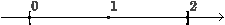
\includegraphics{figures/calculus-errors16} & ${\displaystyle \int_{x_{0}}^{x_{0}+2h}f(x)dx=\frac{h}{3}\left[f(x_{0})+4f(x_{0}+h)+f(x_{0}+2h)\right]+O(h^{5}f^{(4)}(\xi_{h}))}$ & Aturan Simpson\index{aturan Simpson}\tabularnewline
\hline 
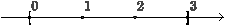
\includegraphics{figures/calculus-errors17} & ${\displaystyle \int_{x_{0}}^{x_{0}+3h}f(x)dx=\frac{3h}{8}\left[f(x_{0})+3f(x_{0}+h)+3f(x_{0}+2h)+f(x_{0}+3h)\right]+O(h^{5}f^{(4)}(\xi_{h}))}$ & Aturan Simpson $\frac{3}{8}$\index{aturan Simpson@aturan Simpson $\frac{3}{8}$}\tabularnewline
\hline 
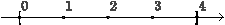
\includegraphics{figures/calculus-errors18} & ${\displaystyle \int_{x_{0}}^{x_{0}+4h}f(x)dx=\frac{2h}{45}\left[7f(x_{0})+32f(x_{0}+h)+12f(x_{0}+2h)+32f(x_{0}+3h)+7f(x_{0}+4h)\right]+O(h^{7}f^{(6)}(\xi_{h}))}$ & Aturan Bode\index{aturan Bode}\tabularnewline
\hline 
\multicolumn{3}{|c}{rumus kuadratur Gauss}\tabularnewline
\hline 
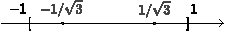
\includegraphics{figures/calculus-errors23} & ${\displaystyle \int_{x_{0}-h}^{x_{0}+h}f(x)dx=h\left[f\left(x_{0}-\frac{1}{\sqrt{3}}h\right)+f\left(x_{0}+\frac{1}{\sqrt{3}}h\right)\right]+O(h^{5}f^{(4)}(\xi_{h}))}$ & \tabularnewline
\hline 
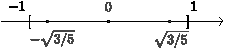
\includegraphics{figures/calculus-errors24} & ${\displaystyle \int_{x_{0}-h}^{x_{0}+h}f(x)dx=\frac{h}{9}\left[5f\left(x_{0}-\sqrt{\frac{3}{5}}h\right)+8f(x_{0})+5f\left(x_{0}+\sqrt{\frac{3}{5}}h\right)\right]+O(h^{7}f^{(6)}(\xi_{h}))}$ & \tabularnewline
\hline 
\end{tabular}
\end{turn}
\end{table}
 merangkum beberapa rumus standar untuk turunan dan integral. Perhatikan
bahwa tidak ada rumus satu titik untuk turunan apa pun, tidak ada
rumus dua titik untuk turunan kedua atau yang lebih tinggi, dan tidak
ada rumus tiga titik untuk turunan ketiga atau yang lebih tinggi.
Stensil telah disederhanakan agar hanya menampilkan nilai $\theta_{i}$.
Dengan demikian, stensil 
\begin{center}
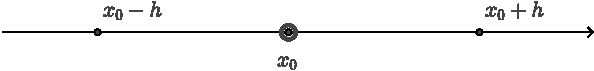
\includegraphics{figures/calculus-rudiments03}
\par\end{center}

\noindent ditampilkan dalam tabel sebagai

\begin{center}
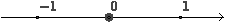
\includegraphics[scale=2]{figures/calculus-errors01}.
\par\end{center}

\subsection{Konsep Kunci}
\begin{description}
\item [{Derajat~ketelitian:~\index{ketelitian!derajat}Bilangan}] bulat
$m$ sedemikian rupa sehingga suatu rumus kalkulus numerik eksak untuk
semua polinom hingga dan termasuk derajat $m$ tetapi tidak eksak
untuk semua polinom berderajat $m+1$.
\item [{Suku~galat:}] Suku galat untuk hampiran kalkulus numerik dapat
ditemukan dengan mengganti setiap kemunculan $f$ dalam rumus hampiran
dengan ekspansi deret Taylor di sekitar $x_{0}$ lalu menyederhanakannya.
\item [{Kuadratur~Gauss:}] \index{kuadratur!Gauss}Metode kuadratur yang
memaksimalkan derajat ketelitian relatif terhadap jumlah simpul yang
digunakan.
\item [{Kuadratur:}] \index{kuadratur}\index{kuadratur|seealso{integrasi numerik}}Nama
lain untuk rumus integrasi numerik.
\item [{Laju~kekonvergenan:~\index{O besar}\index{kekonvergenan!laju}Untuk}] fungsi
$g(h)$ yang memenuhi ${\displaystyle \lim_{h\to0}g(h)=0}$, $p(h)=O(g(h))$
berarti bahwa $|p(h)|\leq M|g(h)|$ untuk suatu konstanta $M$ dan
$h$ yang cukup kecil.
\item [{Teorema~Nilai~Rata-Rata~Berbobot:}] \index{Teorema!Nilai Rata-Rata Berbobot}Asumsikan
bahwa $f$ dan $g$ kontinu pada $[a,b]$. Jika $g$ tidak pernah
berubah tanda dan bernilai nonnegatif pada $[a,b]$, maka berlaku
\[
\int_{a}^{b}f(x)g(x)dx=f(c)\int_{a}^{b}g(x)dx
\]
untuk suatu $c$ di $(a,b)$. 
\end{description}
\begin{small} 

\newpage{}

\subsection{Latihan}
\begin{enumerate}
\item Misalkan $f(x)=e^{x}-\sin x$. Lengkapilah tabel berikut menggunakan
rumus hampiran
\[
f'(x_{0})\approx\frac{-3f(x_{0})+4f(x_{0}+h)-f(x_{0}+2h)}{2h}.
\]

\begin{center}
\begin{tabular}{c|c|c}
$h$ & hampiran $f'(2)$ & galat absolut\tabularnewline
\hline 
$.01$ &  & \tabularnewline
$.005$ &  & \tabularnewline
$-.005$ &  & \tabularnewline
$-.01$ &  & \tabularnewline
\end{tabular}
\par\end{center}

Bolehkah menggunakan nilai negatif untuk $h$?
\item \label{exc:calculusErrors-4} Untuk setiap nilai $x$ dalam tabel,
gunakan rumus tiga titik paling akurat untuk menghampiri $f'(x)$. \hasananswer 

\begin{center}
\begin{tabular}{c|c|c}
$x$ & $f(x)$ & $f'(x)$\tabularnewline
\hline 
$-2.7$ & $0.054797$ & \tabularnewline
$-2.5$ & $0.11342$ & \tabularnewline
$-2.3$ & $0.65536$ & \tabularnewline
$-2.1$ & $0.98472$ & \tabularnewline
\end{tabular}
\par\end{center}
\item \label{exc:calculusErrors}Hampiri integral tersebut menggunakan aturan
Simpson.

\begin{enumerate}
\item \label{exc:calculusErrors-5}${\displaystyle \int_{-0.5}^{0}x\ln(x+1)dx}$ \hasasolution 
\item $\int_{1}^{3}\ln(x+1)\,dx$
\item \label{exc:calculusErrors-6}${\displaystyle \int_{-0.25}^{0.25}(\cos x)^{2}dx}$ \hasananswer 
\item \label{exc:calculusErrors-41}$\int_{1}^{3}e^{\sin x}\:dx$
\item \label{exc:calculusErrors-7}$\int_{1}^{2}x^{4}\,dx$ \hasananswer 
\end{enumerate}
\item \label{exc:calculusErrors-1}Kerjakan soal \ref{exc:calculusErrors}
dengan menggunakan aturan Trapesium. \haspartwithsolution \haspartwithanswer 
\item \label{exc:calculusErrors-2}Kerjakan soal \ref{exc:calculusErrors}
dengan menggunakan Aturan Titik Tengah. \haspartwithsolution \haspartwithanswer 
\item \label{exc:calculusErrors-37}Tentukan galat hampiran pada soal \ref{exc:calculusErrors}.
Anda dapat menggunakan $4.4247999271351$ sebagai nilai eksak integral
pada \ref{exc:calculusErrors-41}. \haspartwithsolution \haspartwithanswer 
\item \label{exc:calculusErrors-38}Tentukan galat hampiran pada soal \ref{exc:calculusErrors-1}.
Anda dapat menggunakan $4.4247999271351$ sebagai nilai eksak integral
pada \ref{exc:calculusErrors-41}. \haspartwithsolution \haspartwithanswer 
\item \label{exc:calculusErrors-39}Tentukan galat hampiran pada soal \ref{exc:calculusErrors-2}.
Anda dapat menggunakan $4.4247999271351$ sebagai nilai eksak integral
pada \ref{exc:calculusErrors-41}. \haspartwithsolution \haspartwithanswer 
\item Tentukan galat dalam menghampiri $\int_{-7}^{11}(32x^{2}+\sqrt{7}x-2)dx$
menggunakan Aturan Simpson $\frac{3}{8}$.
\item \label{exc:calculusErrors-19}Tentukan galat dalam menghampiri $\int_{-17}^{36}(32x^{5}+7x^{3}-2)dx$
menggunakan Aturan Bode. \hasananswer 
\item \label{exc:calculusErrors-3}Untuk nilai $f$, $x_{0}$, dan $h$
berikut, gunakan rumus 
\[
f'(x_{0})=\frac{f(x_{0}+h)-f(x_{0}-h)}{2h}-\frac{h^{2}}{6}f'''(\xi)
\]
untuk menghampiri $f'(x_{0})$.

\begin{enumerate}
\item \label{exc:calculusErrors-36}$f(x)=e^{x}$; $x_{0}=2$; $h=0.1$. \hasasolution 
\item \label{exc:calculusErrors-20}$f(x)=(\cosh2x)^{2}-\sin x$; $x_{0}=\pi$;
$h=0.05$. \hasananswer 
\item $f(x)=\ln(2x-3)+5x$; $x=10$; $h=1$.
\end{enumerate}
\item \label{exc:calculusErrors-8}Hitung batas bawah dan batas atas bagi
galat hampiran pada soal \ref{exc:calculusErrors-3}. Pastikan bahwa
galat sebenarnya berada di antara kedua batas tersebut. \haspartwithsolution  \haspartwithanswer 
\item \label{exc:calculusErrors-9}Untuk setiap bagian soal \ref{exc:calculusErrors-3},
tentukan nilai $\xi$ yang dijamin oleh rumus tersebut. \haspartwithsolution  \haspartwithanswer 
\item Nyatakan derajat ketelitian rumus Newton-Cotes tertutup dengan 5 simpul,
yaitu Aturan Bode.
\item \label{exc:calculusErrors-10}Nyatakan derajat ketelitian rumus lima
titik berikut. \hasasolution 
\begin{align*}
f'(x_{0})=\frac{1}{12h}\left[-25f(x_{0})+48f(x_{0}+h)-36f(x_{0}+2h)\right.\qquad\\
\left.+16f(x_{0}+3h)-3f(x_{0}+4h)\right]+\frac{h^{4}}{5}f^{(5)}(\xi)
\end{align*}
\item Tentukan derajat ketelitian rumus kuadratur
\[
\int_{3}^{5}f(x)\,dx\approx\frac{1}{2}\left[3f\left(\frac{11}{3}\right)+f(5)\right].
\]
\item Tentukan suku galat metode kuadratur tersebut dan nyatakan derajat
ketelitiannya.

\begin{enumerate}
\item \label{exc:calculusErrors-21}${\displaystyle \int_{x_{0}}^{x_{0}+h}f(x)\,dx\approx hf(x_{0})}$ \hasananswer 
\item ${\displaystyle \int_{x_{0}}^{x_{0}+h}f(x)\,dx\approx hf\left(x_{0}+\frac{h}{4}\right)}$
\item \label{exc:calculusErrors-11}${\displaystyle \int_{x_{0}}^{x_{0}+h}f(x)dx\approx\frac{h}{4}\left[3f\left(x_{0}+\frac{2}{3}h\right)+f(x_{0})\right]}$ \hasasolution 
\item ${\displaystyle \int_{x_{0}}^{x_{0}+2h}f(x)dx\approx\frac{h}{2}\left[3f\left(x_{0}+\frac{4}{3}h\right)+f(x_{0})\right]}$
\item \label{exc:calculusErrors-22}${\displaystyle \int_{x_{0}}^{x_{0}+3h}f(x)dx\approx\frac{3h}{4}\left[f(x_{0})+3f(x_{0}+2h)\right]}$ \hasananswer 
\item ${\displaystyle \int_{x_{0}}^{x_{0}+2h}f(x)dx\approx\frac{h}{2}\left[f\left(x_{0}-\frac{h}{2}\right)+3f\left(x_{0}+\frac{3}{2}h\right)\right]}$
\item \label{exc:calculusErrors-23}${\displaystyle \int_{x_{0}}^{x_{0}+2h}f(x)dx\approx\frac{h}{3}\left[f(x_{0}-h)-2f(x_{0})+7f(x_{0}+h)\right]}$ \hasananswer 
\item ${\displaystyle \int_{x_{0}}^{x_{0}+3h}f(x)dx\approx3h\left[3f\left(x_{0}+\frac{3}{2}h\right)-6f(x_{0}+h)+4f\left(x_{0}+\frac{3}{4}h\right)\right]}$
\item \label{exc:calculusErrors-24}${\displaystyle \int_{x_{0}}^{x_{0}+3h}f(x)dx\approx-\frac{h}{12}\left[208f\left(x_{0}+\frac{3}{2}h\right)-891f(x_{0}+h)+1344f\left(x_{0}+\frac{3}{4}h\right)-625f\left(x_{0}+\frac{3}{5}h\right)\right]}$ \hasananswer 
\end{enumerate}
\item Tentukan suku galat hampiran turunan berikut:

\begin{enumerate}
\item \label{exc:calculusErrors-25}${\displaystyle f'(x_{0})\approx\frac{f(x_{0}+2h)-f(x_{0})}{2h}}$ \hasananswer 
\item ${\displaystyle f'(x_{0})\approx\frac{f(x_{0}+2h)-f(x_{0}-h)}{3h}}$
\item \label{exc:calculusErrors-12}${\displaystyle f'(x_{0})\approx\frac{-3f(x_{0})+4f(x_{0}+\frac{h}{2})-f(x_{0}+h)}{h}}$ \hasasolution 
\item ${\displaystyle f'(x_{0})\approx\frac{-13f(x_{0}-10h)-12f(x_{0}+5h)+25f(x_{0}+8h)}{270h}}$
\item \label{exc:calculusErrors-26}${\displaystyle f'(x_{0})\approx\frac{-7f(x_{0}+h)+416f(x_{0}+\frac{1}{2}h)-2916f(x_{0}+\frac{1}{3}h)+5632f(x_{0}+\frac{1}{4}h)-3125f(x_{0}+\frac{1}{5}h)}{12h}}$ \hasananswer 
\item ${\displaystyle f''(x_{0})\approx\frac{2f(x_{0}-h)-3f(x_{0})+f(x_{0}+2h)}{3h^{2}}}$
\item \label{exc:calculusErrors-27}${\displaystyle f''(x_{0})\approx\frac{7f(x_{0}-5h)-12f(x_{0})+5f(x_{0}+7h)}{210h^{2}}}$ \hasananswer 
\item ${\displaystyle f''(x_{0})\approx\frac{5f(x_{0}-5h)-12f(x_{0}+2h)+7f(x_{0}+7h)}{210h^{2}}}$
\item \label{exc:calculusErrors-28}${\displaystyle f''(x_{0})\approx\frac{5f(x_{0}-2h)+32f(x_{0}-h)-60f(x_{0})+25f(x_{0}+2h)-2f(x_{0}+4h)}{60h^{2}}}$ \hasananswer 
\end{enumerate}
\item \label{exc:calculusErrors-17}Diffy Rence menuliskan hampiran berikut:
\[
f''(3.0)\approx25[\sin(2.8)-2\sin(3.0)+\sin(3.2)].
\]

Apa bentuk fungsi $f(x)$? \hasasolution 
\item Misalkan $f(x)=\sin x$. 

\begin{enumerate}
\item Tentukan batas galat untuk hampiran 
\[
f'(6)\approx\frac{-3\sin6+4\sin6.1-\sin6.2}{0.2}
\]
 berdasarkan suku galat yang sesuai.
\item Bandingkan batas ini dengan galat sebenarnya.
\end{enumerate}
\item Apa yang dapat Anda simpulkan tentang galat dalam menghampiri turunan
pertama fungsi 
\[
f(x)=-13x^{4}+17x^{3}-15x^{2}+12x-99
\]
dengan rumus lima titik?
\item Misalkan $f(x)=3x^{3}-2x^{2}+x$.

\begin{enumerate}
\item Hitung galat (bukan batas galat) ketika menaksir $f'(2)$ menggunakan
beda maju
\[
\frac{f(x_{0}+h)-f(x_{0})}{h}
\]
dengan $h=0.1$.
\item Tentukan $\xi_{0.1}$ yang keberadaannya dijamin oleh suku galat.
\end{enumerate}
\item Misalkan $f(x)=\sin x$.  Tentukan batas galat hampiran tersebut.

\begin{enumerate}
\item \label{exc:calculusErrors-29}${\displaystyle f''(3.0)\approx25[\sin(2.8)-2\sin(3.0)+\sin(3.2)]}$ \hasananswer 
\item ${\displaystyle f''(3.0)\approx1600\left[2\sin(3.0)-5\sin(3.025)+4\sin(3.05)-\sin(3.075)\right]}$
\item \label{exc:calculusErrors-13}$f'''(3.0)\approx500000\left[-5\sin(3.0)+18\sin(3.01)-24\sin(3.02)+14\sin(3.03)-3\sin(3.04)\right]$ \hasasolution 
\item ${\displaystyle f'''(3.0)\approx1000\left[-\sin(2.8)+3\sin(2.9)-3\sin(3.0)+\sin(3.1)\right]}$
\item ${\displaystyle \int_{3}^{4}f(x)dx\approx\frac{1}{6}\left[\sin(3)+4\sin(3.5)+\sin(4)\right]}$
\item \label{exc:calculusErrors-14}${\displaystyle \int_{3}^{4}f(x)dx\approx\frac{1}{2}\left[\sin\left(\frac{7}{2}-\frac{1}{2\sqrt{3}}\right)+\sin\left(\frac{7}{2}+\frac{1}{2\sqrt{3}}\right)\right]}$ \hasasolution 
\end{enumerate}
\item \label{exc:calculusErrors-18}Misalkan Anda memiliki data berikut
untuk suatu fungsi $f$. \hasasolution 

\begin{center}
\begin{tabular}{cccccc}
$x$ & $0$ & $1$ & $2$ & $3$ & $4$\tabularnewline
$f(x)$ & $-0.2381$ & $-0.3125$ & $-0.4545$ & $-0.8333$ & $-5$\tabularnewline
\end{tabular}
\par\end{center}
\begin{enumerate}
\item Hampiri $f'(4)$ dan $f'(2)$ menggunakan rumus lima titik. 
\item Menurut Anda, hampiran manakah yang akan lebih akurat, dan mengapa?
\item Apakah hasilnya memang demikian? Data tersebut berasal dari $f(x)=\frac{1}{x-4.2}$.
\end{enumerate}
\item \label{exc:calculusErrors-30}Gunakan metode kuadratur 
\[
\int_{x_{0}}^{x_{0}+h}f(x)\,dx=\frac{h}{2}\left[f\left(x_{0}+\frac{h}{3}\right)+f\left(x_{0}+\frac{2h}{3}\right)\right]+\frac{h^{3}}{36}f''(\xi)
\]
untuk semua pertanyaan berikut. \hasananswer 

\begin{enumerate}
\item Berapakah laju kekonvergenannya?
\item Berapakah derajat ketelitiannya?
\item Gunakan metode tersebut untuk menghampiri $\int_{0}^{\pi}\sin x\,dx$.
\item Tentukan batas galat hampiran ini.
\item Bandingkan batas tersebut dengan galat sebenarnya.
\end{enumerate}
\item Penerapan Aturan Trapesium pada ${\displaystyle \int_{0}^{2}f(x)dx}$
menghasilkan nilai 5, sedangkan Aturan Titik Tengah menghasilkan nilai
4. Nilai berapakah yang diberikan oleh Aturan Simpson?
\item \label{exc:calculusErrors-31}Penerapan Aturan Trapesium pada $\int_{0}^{2}f(x)\,dx$
menghasilkan nilai 4, sedangkan Aturan Simpson menghasilkan nilai
2. Berapakah $f(1)$? \hasananswer 
\item \label{exc:calculusErrors-32}Jika $f'''(x_{0})$ dihampiri menggunakan
lima simpul, berapakah laju kekonvergenan minimalnya?  \hasananswer 
\item Tunjukkan bahwa rata-rata dari hampiran beda maju $\frac{-f(x_{0})+f(x_{0}+h)}{h}$
dan hampiran beda mundur $\frac{-f(x_{0}-h)+f(x_{0})}{h}$ untuk $f'(x_{0})$
menghasilkan hampiran beda terpusat $\frac{f(x_{0}+h)-f(x_{0}-h)}{2h}$
untuk $f'(x_{0})$.
\item \label{exc:calculusErrors-33}Chuck sedang ``menghampiri'' suatu
integral tentu menggunakan Aturan Simpson. Seperti tampak dari pengerjaannya
di bawah ini, ia sedang mengintegralkan polinom kubik. Hitung galat
yang ditimbulkannya meskipun Anda tidak dapat membaca semua koefisiennya. \hasananswer 

\begin{center}
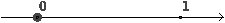
\includegraphics[width=2.5in]{figures/calculus-errors02}
\par\end{center}
\item \label{exc:calculusErrors-40}Ulangi \ref{exc:calculusErrors-33},
kali ini dengan asumsi Chuck menggunakan Aturan Trapesium. \hasananswer 
\item Sketsakan grafik suatu fungsi $f(x)$, lalu tandai nilai $x_{0}$
dan $h$ pada grafik tersebut sedemikian sehingga beda mundur $\frac{f(x_{0})-f(x_{0}-h)}{h}$
menghasilkan hampiran yang \textbf{\emph{lebih baik}} untuk $f'(x_{0})$
daripada beda terpusat $\frac{f(x_{0}+h)-f(x_{0}-h)}{2h}$.
\item \label{exc:calculusErrors-15}Sketsakan grafik suatu fungsi $f(x)$
sedemikian sehingga Aturan Trapesium memberikan hampiran yang lebih
baik untuk $\int_{0}^{1}f(x)\,dx$ daripada Aturan Simpson, lalu jelaskan
bagaimana Anda mengetahuinya. \hasasolution 
\item \label{exc:calculusErrors-16}Misalkan rumus lima titik digunakan
untuk menghampiri $f''(x_{0})$ dengan ukuran langkah $h=0.1$ dan
$h=0.02$. Jika $E_{0.1}$ menyatakan galat hampiran untuk $h=0.1$
dan $E_{0.02}$ menyatakan galat hampiran untuk $h=0.02$, kira-kira
berapakah nilai $\frac{E_{0.1}}{E_{0.02}}$ yang Anda harapkan? \hasasolution 
\item Rumus umum tiga titik yang menggunakan simpul $x_{0}$, $x_{0}+\alpha h$,
dan $x_{0}+2h$, dengan $(\alpha\neq0,2)$, diberikan oleh
\[
f'(x_{0})\approx\frac{1}{2h}\left[-\frac{2+\alpha}{\alpha}f(x_{0})+\frac{4}{\alpha(2-\alpha)}f(x_{0}+\alpha h)-\frac{\alpha}{2-\alpha}f(x_{0}+2h)\right].
\]

\begin{enumerate}
\item Tunjukkan bahwa rumus ini menyederhana menjadi salah satu rumus standar
untuk $\alpha=1$.
\item Tentukan suku galat rumus ini.
\end{enumerate}
\item \label{exc:calculusErrors-34}Tentukan tiga hampiran berbeda untuk
$f'(0.2)$ dengan menggunakan rumus tiga titik. \hasananswer 

\begin{center}
\begin{tabular}{c|c}
$x$ & $f(x)$\tabularnewline
\hline 
$0$ & $1$\tabularnewline
$0.1$ & $1.10517$\tabularnewline
$0.2$ & $1.22140$\tabularnewline
$0.3$ & $1.34986$\tabularnewline
$0.4$ & $1.49182$\tabularnewline
\end{tabular}
\par\end{center}

Grafik $f'''(x)$ ditampilkan di bawah ini. Gunakan grafik tersebut
untuk mengurutkan ketiga hampiran Anda dari yang diperkirakan memiliki
galat terkecil hingga terbesar, lalu jelaskan alasan urutan tersebut.

\begin{center}
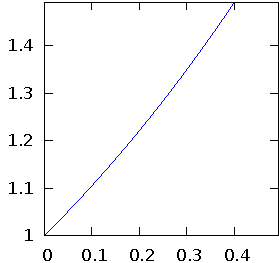
\includegraphics{figures/calculus-errors25}
\par\end{center}
\item Verifikasikan secara numerik bahwa galat saat rumus $f'(x_{0})=\frac{-2f(x_{0}-h)-3f(x_{0})+6f(x_{0}+h)-f(x_{0}+2h)}{6h}$
digunakan untuk menghampiri $f'(3)$ dengan fungsi $f(x)=(\cos3x)^{2}+\ln x$
memang berorde $O(h^{3})$.
\item \label{exc:calculusErrors-35}Dengan komputasi presisi ganda (Octave
standar), tentukan secara numerik taksiran terbaik yang dapat diperoleh
dari rumus 
\[
f'(3)=\frac{-2f(3-h)-3f(3)+6f(3+h)-f(3+2h)}{6h}
\]
 untuk $f(x)=(\cos3x)^{2}+\ln x$. Nilai $h$ berapakah yang menghasilkan
hampiran optimal tersebut? \hasananswer 
\item Tentukan derajat ketelitian rumus kuadratur berikut:
\[
\int_{-1}^{1}f(x)dx=f\left(-\frac{\sqrt{3}}{3}\right)+f\left(\frac{\sqrt{3}}{3}\right).
\]
\item Rumus kuadratur ${\displaystyle \int_{0}^{2}f(x)dx=c_{0}f(0)+c_{1}f(1)+c_{2}f(2)}$
eksak untuk semua polinom berderajat kurang dari atau sama dengan
2. Tentukan $c_{0}$, $c_{1}$, dan $c_{2}$.
\end{enumerate}
\end{small}
